\chapter{Setting up environment}
\label{ch:env_setup}

To set up testing/scenario environment, a special header file \texttt{device.h}, has to be modified. As we can see in Figure \ref{fig:device_h}, all of devices used in program are specified using binary flags which denote their presence/absence in scenario in question.

\begin{figure}[htb]
    \centering
	  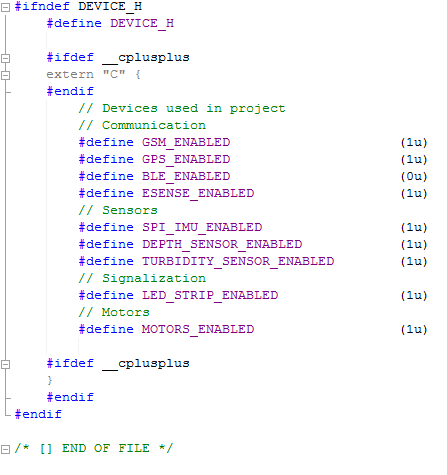
\includegraphics[width=0.7\linewidth]{figures/Environment_setup.PNG}
	\caption{Example setup of device.h}
	\label{fig:device_h}
\end{figure}

In testing scenarios, the most important parameter is \texttt{BLE\_ENABLED} which also specifies the output of debugging messages as well as the expected source of commands. Therefore, if \texttt{BLE\_ENABLED} is set to \texttt{0}, all of the testing is done through wired UART (i.e. USB cable), otherwise the input is expected to come from BLE device.